\chapter*{Existe resistência nas sociedades de controle?\\ \emph{\small{A reação social diante da apropriação da rede pela lógica do capital}}}

\addcontentsline{toc}{chapter}{Existe resistência nas sociedades de controle?}

\begin{flushright}
\emph{Mariella Batarra Mian}\footnote{Doutorado em andamento no programa de
  pós-graduação em Ciências Humanas e Sociais pela Universidade Federal
  do ABC - UFABC. Mestre pelo mesmo programa da UFABC. Especialista em
  Gestão de Marketing pela Fundação Armando Álvares Penteado - FAAP.
  Graduada em comunicação social - habilitação em Relações Públicas,
  pela Universidade Estadual Paulista - UNESP. Atua como Relações
  Públicas na Universidade Federal do ABC.\\
  E-mail: \emph{mariellabm@gmail.com}.}
\end{flushright}

\section{Introdução}

A sociedade é constituída, fundamentalmente, pela constante interação
entre os indivíduos em entidades por eles formadas, dentre as quais:
familiares, políticas, educacionais, legislativas, religiosas, de
trabalho, culturais, ambientais, econômicas, e outras. Essa
indissociável convivência entre atores é o pressuposto da condição
social e é tangenciada por intrínsecas relações de poder, sejam aquelas
hierarquicamente formalizadas - chefes de Estado \emph{versus}
população, empregadores \emph{versus} empregados, líderes religiosos
\emph{versus} seguidores religiosos etc. -- às violentamente
explicitadas -- como quando há abusos por parte de instituições oficiais
de segurança e em regimes ditatoriais, com a naturalização de situações
com tortura humana - ou, ainda, aquelas relações em que o poder está
simbolicamente estabelecido (Bourdieu, 1989) -- geralmente invisível,
guardado nas entrelinhas, por meio de discursos e violências
psicológicas. Este tipo de poder é comumente destacado na
contemporaneidade ao tratar-se de temas como machismo, homofobia,
racismo etc.

O componente inseparável deste poder, tão evidenciado nas relações
sociais, é exatamente o seu legítimo contraponto: a resistência.
Trata-se de um vínculo dialético, quase que interdependente. A
resistência, em suas formas mais tradicionalmente reconhecidas -- como
são as grandes revoluções da história humana -, apresenta-se como o
combustível para mudanças de paradigmas na sociedade.

Contudo, além dessas formas mais enfáticas e notáveis de resistência,
este contrapoder é exercido mais comumente em suas formas mais brandas.
Ainda que não sejam tão explícitas nas relações sociais, essas
denominadas formas de resistências cotidianas (Scott, 1985) exercem
importantes formas de oposição e de reação aos mais diversos e
corriqueiros tipos de poder que permeiam a sociedade. Dentre outros
exemplos, pequenas ações de desobediência em contextos de trabalho podem
ser retratadas como típicos exemplos dessa resistência cotidiana.

De modo geral, é a partir do prevalecimento dos interesses de
determinados entes sociais, em detrimento do interesse de outros, que
emergem os mais diversos tipos de ações de resistência, como propulsoras
do antagonismo ao poder.

No contexto contemporâneo, permeado pelas tecnologias de informação e
comunicação (TICs), a sociedade vem lidando com inúmeras transformações.
Com a chegada da internet ocorreram mudanças expressivas nos meios de
interação social, principalmente a partir da década de 1990, quando esse
fenômeno transcendeu seus objetivos militares e começou a ser
incorporado pela sociedade como um todo.

Essa realidade informacional impulsionou a forma de articulação dos
indivíduos e ampliou a capacidade dos usuários em utilizarem as redes
sociais online, como forma de expressar livremente suas ideias, e de se
aproximarem ativamente de questões globais de âmbitos políticos,
econômicos, culturais, sociais e ambientais.

Entretanto, como era de se esperar, a lógica do capital desvendou a
dinâmica das redes online e vem se apropriando com destreza dessa
ferramenta. As consequências já são notáveis: pela incessante coleta de
dados pessoais dos usuários, a privacidade tem se tornado algo raro aos
indivíduos da contemporaneidade, trata-se das denominadas sociedades de
controle (Deleuze, 1990). Diante dessa realidade, a proposta deste
trabalho é compreender quais seriam as possíveis ações de resistência
dos indivíduos que buscam contrapor esta nova forma de poder e controle
social. Para tanto, será apresentada, a seguir, a concepção da sociedade
informacional e de controle da contemporaneidade, em seguida, serão
abordados os conceitos sobre as formas de resistência social, e,
finalmente, serão postas as reflexões sobre possíveis ações de
resistência engendradas no contexto atual.

\section{Sociedade contemporânea: informacional e de controle}

Ainda que a exclusão digital seja assunto de extrema relevância,
principalmente sob a ótica dos direitos humanos, é evidente que a
internet assumiu um papel protagonista na sociedade contemporânea. Sua
exponencial abrangência, em nível global, trouxe uma valorização das
relações entre pessoas-pessoas e pessoas-máquinas.

Um dos principais teóricos que se debruça a compreender a dinâmica dessa
realidade é o sociólogo catalão Manuel Castells. Já, em 1999, ele cunha
o termo ``Sociedade Informacional'', baseando-se na fusão dos
significados referentes às expressões ``sociedade da informação''- a
qual está relacionada à ideia da inovação tecnológica - e ``sociedade do
conhecimento'' - que adiciona uma dimensão de transformação social,
cultural, econômica e política.

Ainda no final da década de 1990, o pesquisador relacionou a dinâmica
social operada pelas redes online a um novo modelo de capitalismo, em
que as TICs seriam responsáveis por reconfigurar o sistema produtivo no
denominado ``capitalismo informacional'' (Castells, 1999).

A interação entre os indivíduos e esse espaço virtual informacional
engendra a cultura da recombinação de conteúdos -- cibercultura - e
reforça a clássica teoria social de Marcel Mauss (2003) sobre a
``dádiva'', em que a ininterrupta e concomitante relação de troca
estabelecida entre os atores sociais -- o dar, o receber e o retribuir
-- é evidenciada como o fato social total. Trata-se de um princípio
universal da sociedade: a reciprocidade. Ou seja, muito antes da chegada
da internet, a troca de saberes, de sentimentos, de cultura e de matéria
entre os indivíduos já era reconhecida como algo inerente à construção
social.

No contexto contemporâneo, Wellman, Côte e Plickert (2006) reforçam esse
princípio da troca como indissociável da natureza da cibercultura, é o
cerne do que o compartilhamento em rede representa. Em outras palavras,
a reciprocidade traduz essencialmente o que é a sociedade informacional.
Rainie e Wellman (2012, p.218) enfatizam que:

\begin{quote}
Trocas recíprocas de informação e de interação social é regra entre
aqueles que utilizam as TICs (Tecnologias de informação e comunicação).
Ao mesmo tempo em que criam conteúdos, os usuários estão frequente e
intimamente envolvidos em negociar com seus pares por meio dessa norma
social. (Rainie e Wellman, 2012, 218, tradução nossa) \footnote{Citação
  original: Reciprocal exchanges of information and social interaction
  are the norm among those who use ICTs {[}information and communication
  technologies{]}. As they are creating content, users are often
  intimately involved in bargaining with their peers over social
  niceties}.
\end{quote}

Os pontos apresentados até o momento demonstram como as redes online
reconfiguraram a dinâmica da sociedade, transformando a forma de
organização social contemporânea. Torna-se relevante, a partir deste
ponto, problematizar outras complexas questões e incongruências
relacionadas à internet, sociedade, democracia, direitos humanos, poder
e controle.

A arquitetura das redes online segue uma lógica horizontal e está em
permanente alteração por intermédio das interações ininterruptas e
constante troca de informações entre os atores nelas conectados. Essa
estrutura, amparada por uma série de aportes tecnológicos, emerge na
contemporaneidade, como uma ferramenta com grande potencial, para
favorecer os processos democráticos, amplificar as vozes dos indivíduos
e permitir novos desenhos participativos na arena política. (Araújo,
Penteado e Santos, 2015).

Contudo, mesmo que na internet prevaleça essa lógica de liberdade,
deve-se ter em mente que a rede mundial de computadores está inserida na
sociedade e faz parte de um contexto social hierarquizado, regulado em
muitos (ou em todos os) aspectos por poderes do Estado, da Igreja, do
Mercado, organizações etc. Dessa forma, essa ideia de que a Internet
atua paralelamente ao controle de tais instituições é utópica. Assim,
``a linguagem básica da sociedade da informação pode ser privada ou
pública, fechada ou aberta, hierarquicamente construída ou
compartilhada, obscura ou transparente, enfim, democrática ou
autoritária'' (Silveira, 2005, 13).

O conceito de ``Poder nas Redes'', elucidado pelo teórico Manuel
Castells (2010), busca definir os processos concretos de exercício de
poder na rede. Para o sociólogo catalão, o poder refere-se à capacidade
relacional que permite que determinada entidade influencie, de maneira
assimétrica, as decisões de outros atores sociais, de modo que sejam
favorecidas a vontade, interesses e valores deste ente detentor do
poder. Para o teórico catalão, uma das formas de se exercer o poder e
controlar o outro na internet ocorre por meio da ``capacidade de
estabelecer redes e de programar/ reprogramar redes de acordo com os
objetivos que lhes são atribuídos'' (Castells, 2009, 76, tradução nossa)
\footnote{Citação original: ``la capacidad de constituir redes y de
  programar/reprogramar las redes según los objetivos que se les
  assignen''}.

Para compreender a dinâmica do exercício do poder nas redes online,
torna-se relevante visitar a teoria denominada ``ator-rede'', de Bruno
Latour (2010). Essa perspectiva teórica compreende a sociedade como rede
heterogênea formada por entes humanos e não humanos (materiais), por
ideias e conceitos.


\begin{figure}[!ht]
%\begin{minipage}{0,4\textwidth}
\centering
  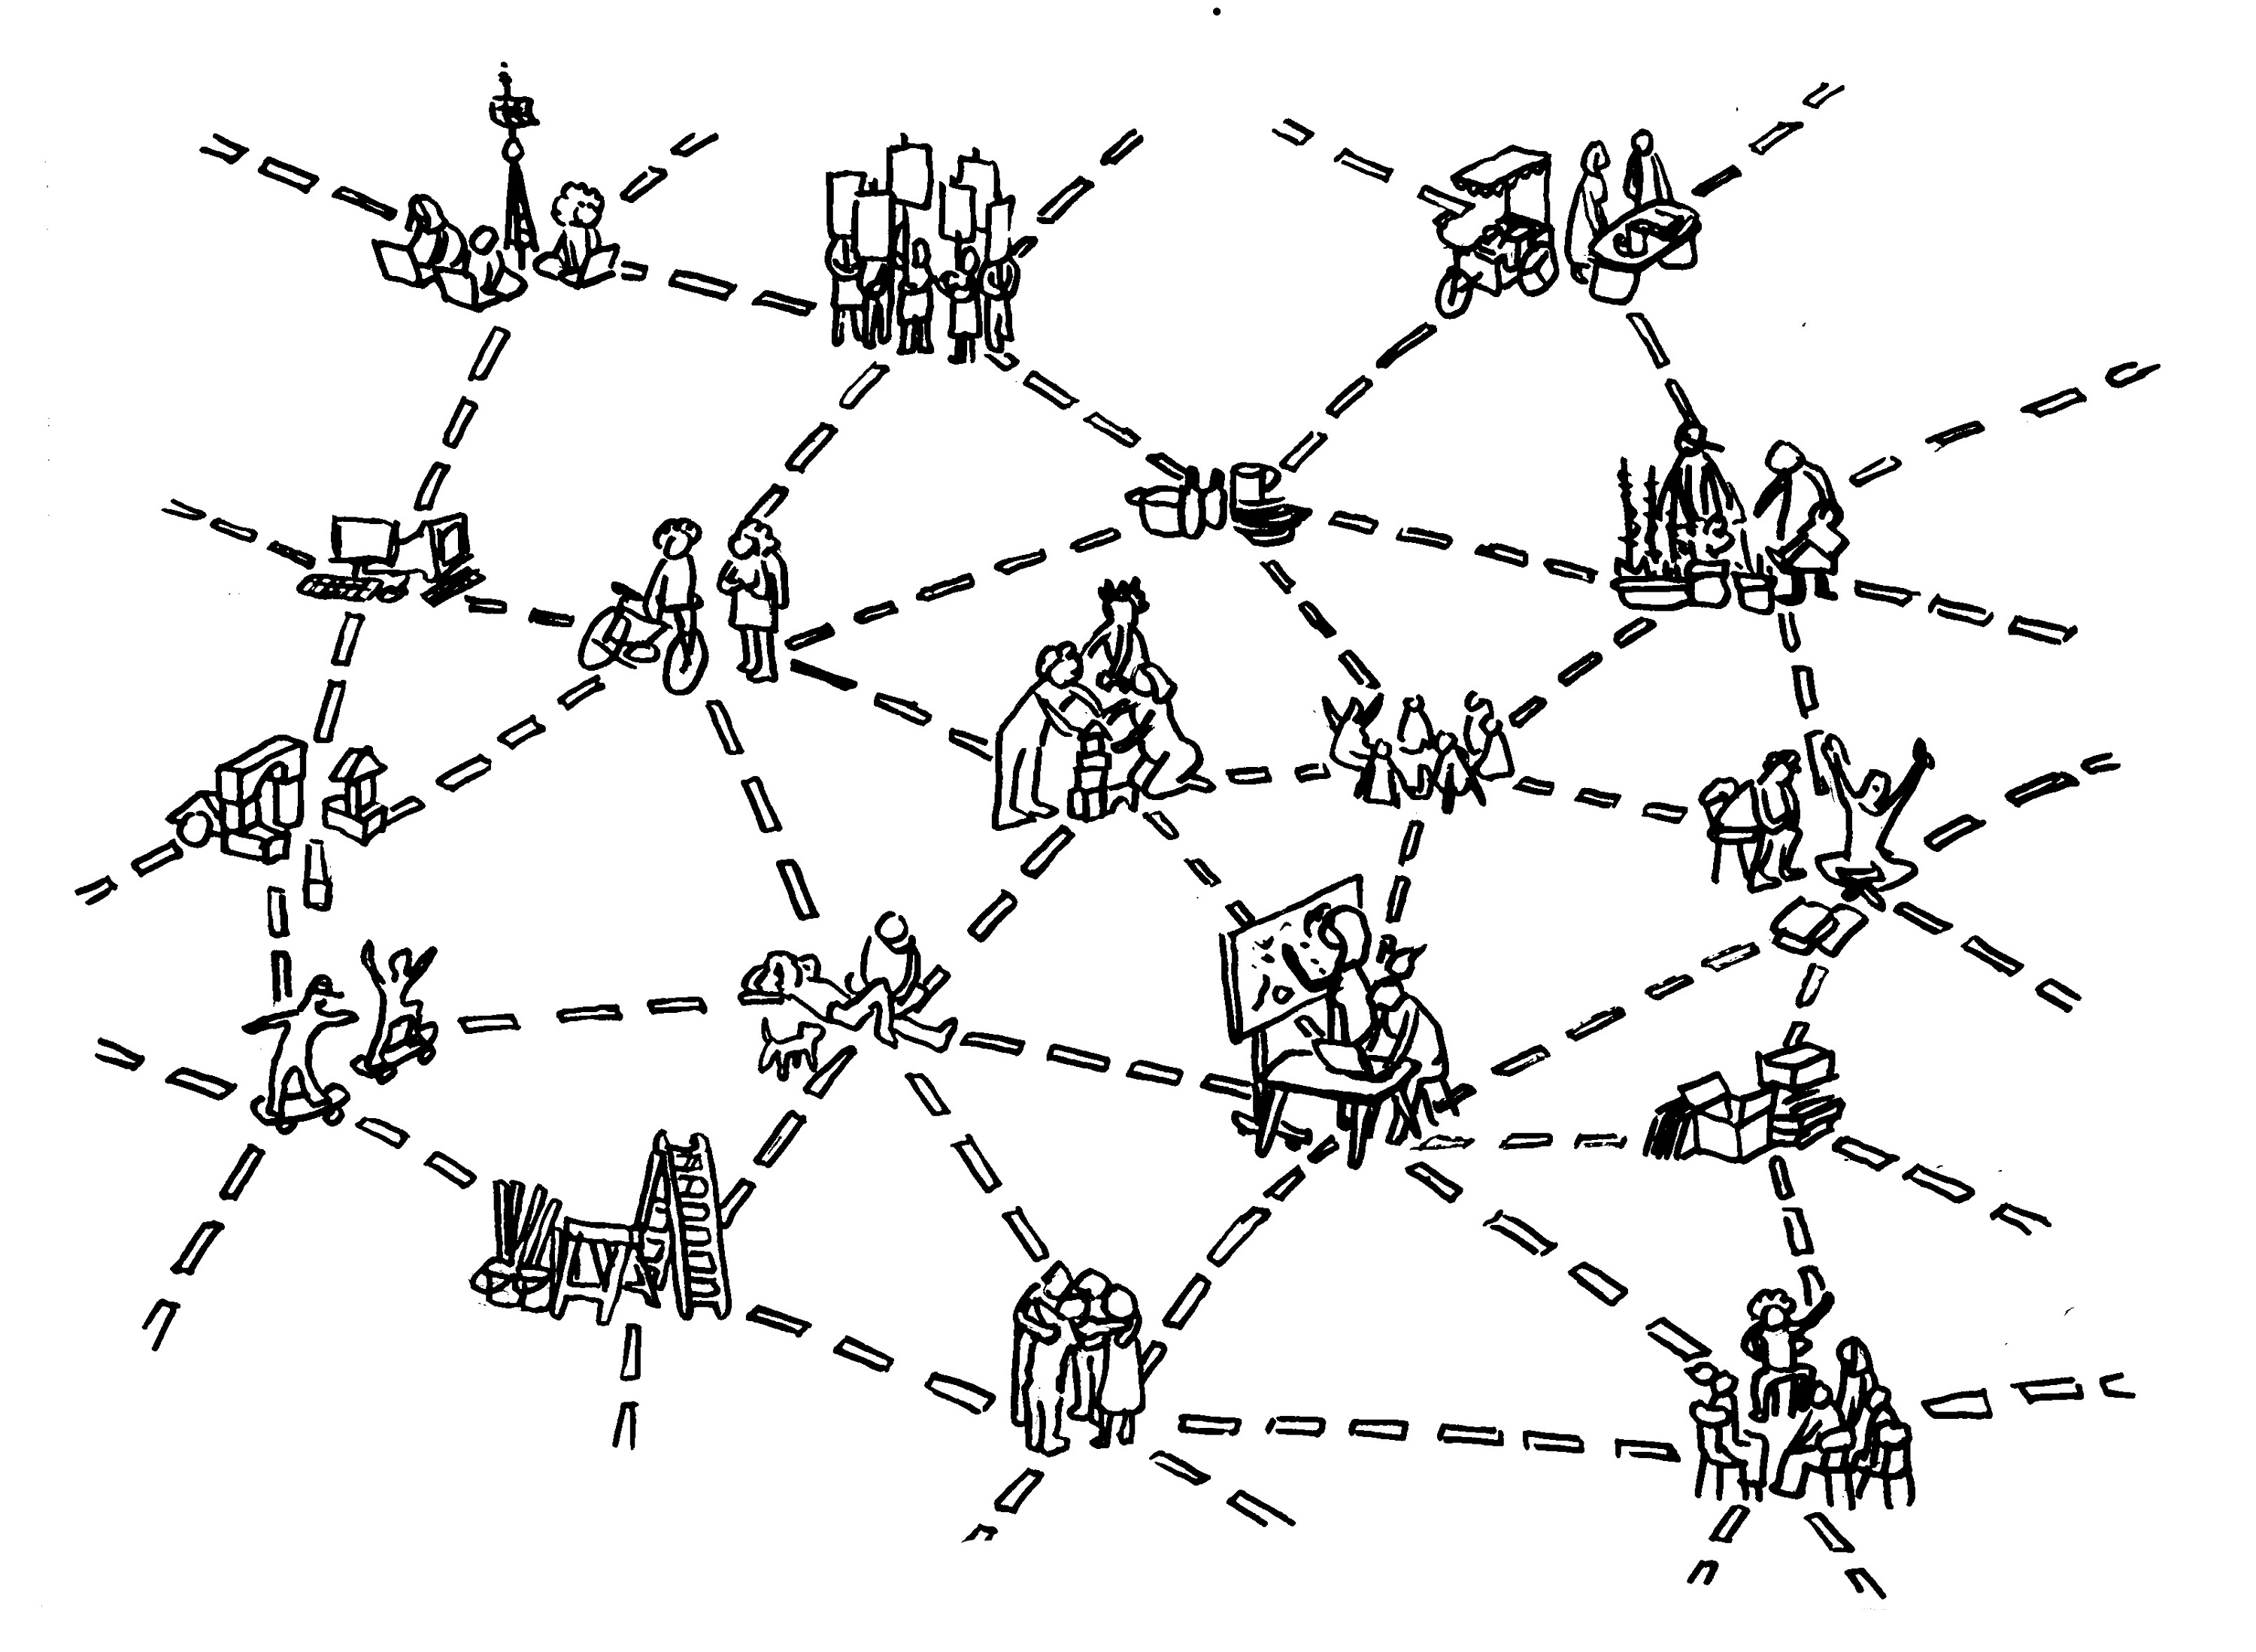
\includegraphics[width=80mm]{./imgs/grafico4.jpg}
\caption{Figura 3 -- Ilustração baseada na Teoria do Ator-Rede de Bruno Latour (Wikimedia, 2018)}
%\end{minipage}
 \end{figure}

A figura 3 demonstra a organização em rede considerando a teoria de
Latour (2010). Nela, é possível observar a diversidade de entes que
constituem a rede. São os chamados ``actantes'', que, ao mesmo tempo em
que assumem identidades singulares na rede, são dependentes das
inter-relações que estabelecem entre si para garantir sua existência na
rede.

A perspectiva teórica de Latour também traz um diálogo com a já
mencionada Teoria da Dádiva de Marcel Mauss (2003), ao considerar que,
além dos elos entre os próprios atores sociais, a sociedade é
constituída, também, por elos estabelecidos entre indivíduos, coisas e
simbolismos.

Para exemplificar a operação do poder na rede, Castells (2009) dialoga
com a teoria elucidada por Bruno Latour (2010):

\begin{quote}
{[}...{]} Sugiro que, em muitos casos, aqueles que detêm o poder são,
também, rede. Não redes abstratas ou inconscientes e nem mecânica: são
seres humanos organizados em torno de seus projetos e interesses. Mas
eles não são elementos isolados (indivíduos, grupos, classes, líderes
religiosos ou políticos), já que o exercício do poder na sociedade em
rede requer um complexo grupo de ação conjunta que transcende as
alianças para se tornar uma nova forma de sujeito, semelhante ao que
Bruno Latour descreveu brilhantemente como "ator-rede"\footnote{Citação
  original: {[}...{]} sugiero que , em muchos casos, quines ostentan el
  poder son, también, red. No redes abstractas e inconscientes ni
  autómatas: se trata de seres humanos organizados alrededor de sus
  proyectos y interesses. Pero no son acotres aislados (individuos,
  grupos, clases, líderes religiosos o políticos), ya que el ejercicio
  del poder en la sociedad red requiere um complejo grupo de acción
  conjunta transciende las alianzas hasta convertirse en una nueva forma
  de sujeto, similiar a lo que Bruno Latour ha descrito btillantemente
  como "actor-red''} (Castells, 2009, 76, tradução nossa)
\end{quote}

No contexto da sociedade contemporânea, intermediada pelas TICs, esse
poder de controlar a rede tem sido amplamente apropriado por aqueles que
tradicionalmente detêm o domínio na sociedade. Grosso modo, pode-se
dizer que a força do capital desvendou as nuances dessa rede horizontal,
favorável à democracia, e vêm demonstrando indiscutível habilidade em se
apossar de sua lógica para fortalecer sua estrutura vertical e
desagregadora. A rede foi cooptada pelos donos do capital, apropriada
pela grande indústria infocomunicacional e é articulada por agências de
marketing.

A conjuntura social vigente foi definida por Deleuze (1990) como
``sociedades de controle''. Trata-se de um momento em que as formas
disciplinares, pautadas pela introjeção do medo à punição e consequente
submissão dos comportamentos (Foucault, 2004), vêm sendo superadas
gradativamente pelos controles cibernéticos. Estes controles são
exercidos, essencialmente, por meio dos inúmeros aparatos tecnológicos
que cercam a vida cotidiana dos indivíduos da atualidade, especialmente
os \emph{smartphones.} De acordo com Silveira (2017, p. 161), os
controles cibernéticos: ``acompanham as pessoas em suas trajetórias, dão
a sensação de conforto, são eficazes na solução de problemas, melhoram
as experiências e não geram medo, mas sim, afeto.''.

Para o teórico Maurizio Lazzarato (2006), as sociedades de controle
caracterizam-se pela multiplicação da oferta de ``mundos'' aos
indivíduos. Nesse sentido, o pesquisador considera as ``máquinas de
expressão'' e as potentes ações de marketing como principais
responsáveis por essa criação e propagação de mundos na sociedade.

Essa ideia de acesso a múltiplas realidades traz a sensação de liberdade
às pessoas. Trata-se, no entanto, de uma ilusão, visto que os seres
humanos estão limitados a se encaixar em mundos criados pelo próprio
sistema capitalista e não há possibilidades de criar mundos próprios.

Nesta realidade, o conceito de modulação é potencializado. Não se trata
mais de manipular opiniões dos indivíduos. O perfil de cada pessoa é
minuciosamente traçado para que os comportamentos humanos ocorram com
propósitos de consumo sistematizados.

\begin{quote}
Os processos de modulação não são meramente de distribuição de
publicidade, eles implicam a construção de situações sociais, de
interações específicas, criando ambientes completamente distintos
daqueles em que a propaganda é realizada nos intervalos dos espetáculos
ou eventos esportivos televisionados. As tecnologias de modulação
permitem agir de modo eficaz sobre nossa atenção por serem quase sempre
baseadas em nossa subjetividade revelada e em nosso potencial afetivo.
(Silveira, 2017, p.150-151).
\end{quote}

Um dos pontos mais críticos em relação a essa operação do poder nas
redes online refere-se à ininterrupta e colossal coleta de dados
pessoais. Sob a prerrogativa de entreter e facilitar o cotidiano dos
usuários das redes, por meio da infinita oferta de serviços e das
inúmeras possibilidades de interação, via redes online e via aplicativos
em dispositivos móveis, as grandes corporações e agências de marketing
vêm atuando com afinco nesse mercado, que representa e já evidência
riscos explícitos a direitos humanos fundamentais: a privacidade e o
anonimato. Nas palavras do sociólogo Sérgio Amadeu da Silveira (2017):

\begin{quote}
O direito à privacidade, além de ser essencial para as democracias, uma
vez que assegura a comunicação e as articulações dos frágeis diante dos
vários grupos de poder, adquiriu uma dimensão econômica no cenário
informacional qualitativamente distinta da existente no mundo
industrial. Os dados pessoais e aqueles que permitem identificar uma
pessoa devem ser considerados parte da identidade pessoal. Portanto, seu
uso exige autorização, o seu tratamento econômico exige
negociação.(Silveira, 2017, p.171-172).
\end{quote}

As eleições de 2016, nos Estados Unidos, e as recentes
polêmicas\footnote{Diversas notícias foram repercutidas na mídia. O
  veículo ``El País'' elaborou uma página na internet com uma série de
  reportagens relacionada a essa temática.} envolvendo a venda de dados
dos usuários da maior plataforma de relacionamento online, Facebook,
para a empresa britânica de marketing político, \emph{Cambridge
Analytica}\footnote{Empresa utiliza tecnologia baseada em
  microsegmentação de dados, para avaliar a personalidade das pessoas a
  partir das pegadas digitais e promover campanhas de marketing
  político.}\emph{,} evidenciaram ainda mais o negligente esquema do
mercado de dados pessoais e escancaram a fragilidade da privacidade dos
indivíduos.

Diante do exposto neste tópico, é possível compreender que a dinâmica de
operação da sociedade informacional, permeada pelas redes online, também
é constituída por relações de poder e resistência que perduram na
história da humanidade. Observa-se que, ainda que a internet seja uma
tecnologia com potencial libertário e democrático, na mesma medida, ela
também pode estar a serviço do controle oculto e, portanto, mais
invasivo aos indivíduos.

A partir deste retrato da realidade, surge um instigante questionamento
acerca das possíveis reações partindo desses cidadãos -- controlados e
modulados -- em relação a essa nova forma de operação do poder. Enquanto
nas sociedades disciplinares os dominadores eram identificáveis e o
embate dos dominados era direcionado com especificidade, nas sociedades
de controle o poder está dissolvido e adocicado. Trazendo uma relação
com as proposições de Bauman (2001) sobre os tempos atuais, é possível
assumir que, na contemporaneidade, o alvo é líquido. Assim, faz-se
necessária uma reflexão acerca das possíveis ações de resistência que
contrapõem essa liquidez do poder na conjuntura contemporânea.

\section{Resistência, o pressuposto do poder}

De acordo com as proposições já apontadas neste texto, compreende-se que
a sociedade é permeada pelas relações de poder. Nesse sentido, torna-se
essencial discorrer sobre o pressuposto fundamental existente nessas
relações: a resistência. Nas palavras de Foucault: ``lá onde há poder há
resistência e, no entanto (ou melhor, por isso mesmo) esta nunca se
encontra em posição de exterioridade em relação ao poder''. (Foucault,
2001, 91).

No âmbito das ciências sociais, o termo ``resistência'' permite
diferentes formas de compreensão. Considerando o viés mais amplamente
difundido e reconhecido, a resistência social carrega um sentido
enfático e com práticas evidentes de antagonismo ao sistema vigente. São
ações com grande repercussão -- como as revoluções -- que legitimam
transformações e rupturas históricas. Os movimentos sociais são
representações explícitas de enfrentamento ao poder.

No decorrer da história ocorreram diversos movimentos sociais que
delinearam os caminhos da humanidade. Para Maria da Glória Gohn (2011),
esses movimentos sociais sempre existiram e sempre existirão. A teórica
acredita que essas ações coletivas ``são o coração, o pulsar da
sociedade. Eles expressam energias de resistência ao velho que oprime ou
de construção do novo que liberte.'' (Gohn, 2011, 336).

Para o sociólogo Manuel Castells (1999) as ações de resistência são as
mais importantes e eficazes maneiras de construção da
identidade\footnote{O conceito de ``identidade'' considerado pelo autor
  refere-se ``a fonte de significado e experiência de um povo''} social.
O sociólogo acredita que os movimentos sociais são ``ações coletivas com
um determinado propósito cujo resultado, tanto em caso de sucesso como
de fracasso, transforma os valores e instituições da sociedade''
(Castells, 2000, 20).

Contudo, sem desconsiderar a relevância dessas formas de resistência que
geralmente possuem caráter institucionalizado, coletivo e
político-partidário, há outras formas de manifestação da resistência
social, inclusive, mais corriqueiras do que aquelas formalizadas.

Os esforços empíricos e teóricos do pesquisador James Scott, que se
aprofundou em estudos sobre a vida camponesa, trazem importantes
reflexões sobre o que ele denomina como ``formas cotidianas de
resistência''. Sobre as elucidações do teórico, Menezes (2002, 33)
afirma que: ``Scott entende que, na maioria das vezes, a resistência às
relações de dominação expressa-se em práticas cotidianas e discursos
difusos, fragmentados, que orientam as interações cotidianas entre
dominantes e dominados.''

Assim, considerando esse viés apresentado por Scott, é possível
compreender que as formas de resistência podem ser manifestadas de
diversas formas pelos indivíduos. Nas palavras do próprio pesquisador:

\begin{quote}
Aqui tenho em mente as armas comuns dos grupos relativamente sem poder:
fazer ``corpo mole'', a dissimulação, a submissão falsa, os saques, os
incêndios premeditados, a ignorância fingida, a fofoca, a sabotagem e
outras armas dessa natureza. Essas formas brechtianas de luta de classe
têm certas características em comum: requerem pouca ou nenhuma
coordenação ou planejamento; sempre representam uma forma de auto-ajuda
individual; evitam, geralmente, qualquer confrontação simbólica com a
autoridade ou com as normas de uma elite. (Scott, 2002, 11-12)
\end{quote}

Outra proposição de Scott, analisada por Menezes (2002, 33), expõe que o
teórico discorda da separação entre `resistência real' e `resistência
incidental' e considera como formas de resistências, igualmente
relevantes à sociedade, tanto as práticas cotidianas, quanto as dos
movimentos sociais, estando até mesmo relacionadas em determinados
contextos. Entretanto, somente em caráter de classificação, Scott (1985,
\emph{apud}, Menezes, 2002) propõe a distinção conceitual entre essas
formas de resistência:

\begin{quote}
Resistência real, se argumenta, é (a) organizada, sistemática e
cooperativa; (b) guiada por princípios e não-egoísta; (c) tem
consequências revolucionárias e /ou (d) incorpora ideias ou intenções
que negam as bases da dominação em si mesmas. Atividades incidentais ou
epifenomênicas, por contraste, são (a) desorganizadas, não-sistemáticas
e individuais; (b) oportunistas e de auto-satisfação; (c) não têm
consequências revolucionárias e/ou (d) implicam na sua intenção ou
significado, uma acomodação com o sistema de dominação (p.33).
\end{quote}

As abordagens sobre essas formas cotidianas de resistência revelam
algumas reflexões interessantes. No que tange suas formas de atuação,
nem sempre são identificáveis. Muitas vezes estão presentes em discursos
ocultos ou em sutis ações de desobediência. E justamente por não
representarem o contrapoder com nitidez, como fazem os movimentos
sociais, por exemplo, recaem alguns questionamentos sobre essas ações
cotidianas, que contestam sua capacidade de transformação do contexto
social e polemizam, inclusive, o uso do termo ``resistência'' para
caracterizá-las. Uma problematização interessante refere-se a uma
provável ambiguidade abarcada na conceituação. Nesse sentido, Menezes
(2002) reflete que:

\begin{quote}
É inegável que a análise destas práticas {[}de resistências
cotidianas{]} abre perspectivas de compreender a política de grupos
subalternos para além da noção de hegemonia ou de conformismo e
passividade. Mas, muitas vezes, elas apenas amenizam a indignação a que
indivíduos e grupos estão submetidos, não alterando, substancialmente,
as relações de dominação. Assim, há o perigo de romantizar a resistência
cotidiana, esquecendo-se de que ela também contribui para a reprodução
das relações de dominação (p.43).
\end{quote}

Contudo, ainda que o conceito possibilite problematizações, ele abarca
uma importante perspectiva acerca das relações de poder que permeiam a
sociedade. Trata-se de uma definição que necessita transcender o campo
teórico e partir substancialmente para o campo prático de análise
(Menezes, 2002).

A grande contribuição trazida por Scott, ao analisar as formas de
resistências cotidianas, revela-se na premissa de sempre considerar a
capacidade de agência dos atores sociais. Ou seja, para o teórico, mesmo
que estejam vivendo situações extremas de controle social, os seres
humanos não perdem seu potencial em delinear as formas de enfrentamento,
ainda que essa resistência exerça-se por meio de pequenas atitudes --
que se confundem, inclusive, com certa passividade.

Diante do exposto acerca desse pressuposto que permeia as relações
sociais de poder, qual seja, a resistência, serão problematizados, a
seguir, os apontamentos quanto às prováveis formas de contrapoder
assumidas pelos atores inseridos nessa sociedade informacional e de
controle.

\section{Resistência na sociedade contemporânea}

As peculiaridades da sociedade contemporânea, informacional e de
controle, trouxeram novas reflexões sobre as ações de resistência
social. O final da primeira década deste século foi marcado por uma
mudança no modo de organização dos movimentos sociais. Essa típica forma
de resistência da contemporaneidade foi denominada ``Ciberativismo''
(Ugarte, 2008) e evidenciou a capacidade da rede em engajar indivíduos
em prol de causas públicas e políticas.

O teórico Manuel Castells, em sua obra ``Redes de Indignação e
Esperança'', explicita as principais características dos movimentos
sociais articulados pela rede e aponta os fatores que os diferenciam dos
movimentos tradicionais. Para o teórico:

\begin{quote}
``Os movimentos sociais em rede de nossa época são amplamente
fundamentados na internet, que é um componente necessário, embora não
suficiente, da ação coletiva. As redes sociais digitais baseadas na
internet e nas plataformas sem fio são ferramentas decisivas para
mobilizar, organizar, deliberar, coordenar e decidir. Mas o papel da
internet ultrapassa a instrumentalidade: ele cria as condições para uma
forma de prática comum que permite a um movimento sem liderança
sobreviver, deliberar, coordenar e expandir-se. (Castells, 2013, 478)
\end{quote}

Diante do contexto em que estavam inseridos é natural que Ugarte (2008)
e Castells (2013), reconhecendo o potencial inerente das redes, tenham
expostos com mais confiança seus pontos de vista sobre a participação e
mobilização cidadã nessa ``esfera pública interconectada'' (Benkler,
2006).

Ademais, é importante considerar que a internet já foi palco para a
concretização de representativos movimentos sociais que movimentaram
estruturas de poderes verticais consolidados ao redor do mundo. É o caso
da ``Primavera Árabe'', ``Occupy Wall Street'', ``15M'' e, no contexto
brasileiro, os movimentos de ``junho 2013'', (Mian e Zotelli, 2016).
Quanto a caracterização, as referidas formas de resistência em rede,
mesmo que evidenciem grandes diferenças de formulação em relação aos
movimentos sociais tradicionais (aqueles iniciados no ambiente
off-line), também se caracterizam por serem ações mais estruturadas de
contrapoder.

Esse ciberativismo amplia a voz de muitos atores sociais e pode ser
considerado uma das formas de exercício do contrapoder na sociedade
contemporânea. Contudo, após a lógica da internet ter sido compreendida
e, principalmente, cooptada pelo capital, essa forma de resistência vem
reduzindo seu potencial de impacto junto às estruturas de poder.

Os movimentos sociais articulados em rede ainda existem, e a lógica da
internet ainda é um importante subsídio para a organização de suas
ações, contudo, o caráter espontâneo dessas mobilizações -- que nos
movimentos acima citados foi o principal provocador e desestabilizador
do sistema -- não possui força para driblar a lógica vertical do poder.

Como já explicitado, o poder de controlar as redes, por meio da coleta
de dados pessoais e da venda de perfis de usuários para fins de
publicidade, é a prerrogativa de atuação das grandes corporações do
mundo, as chamadas organizações de infocomunicação. Dentre as
principais, destacam-se: Google, Apple e Facebook. Portanto, é
praticamente inevitável, a qualquer usuário comum de internet, utilizar
a rede sem se conectar a plataformas que não estejam vinculadas a pelo
menos uma dessas três corporações.

A hiperconectividade do mundo torna-se, portanto, diretamente
proporcional à vulnerabilidade dos dados pessoais e, consequentemente,
da privacidade dos indivíduos. É justamente esta escancarada invasão da
vida intima dos indivíduos o contraponto central dessa nova lógica de
operação do poder.

A privacidade é reconhecida mundialmente como um dos direitos humanos
fundamentais (IRPC, 2018). No Brasil, é um direito fundamental, previsto
no inciso X do artigo quinto da Constituição de 1988. (BRASIL, 2018)
Assim, torna-se relevante a discussão sobre as possíveis formas de
resistência social em um cenário em que um direito básico é violado e
posto em xeque initerruptamente.

Tal problematização tem chamado a atenção de diversos grupos que assumem
posicionamentos antagônicos à referida conjuntura. Nesse sentido, é
possível elencar algumas ações coordenadas e institucionalizadas que
formalizam resistência a essa lógica de controle das redes. Assim como
os movimentos sociais articulados em rede, tratam-se também de
engajamentos sistematizados contra o poder, cujos objetivos são bem
definidos, é a resistência real às sociedades de controle.

Um dos grandes ativistas que atua formalmente nas redes é o mundialmente
reconhecido ``Anonymous''. Conforme Machado (2013), mais do que um
grupo, ou um conjunto unificado e formal de indivíduos, o ``Anonymous''
deve ser reconhecido como ``uma ideia'' e justamente ``por se tratar de
uma ideia, não conta com donos, liderança central e muito menos centro
geográfico'' (p.21).

Essa rede Anonymous já protagonizou inúmeras ações contrapondo líderes
de estado e declarando apoio aos direitos humanos nas redes. O Anonymous
é também um grande incentivador do uso de plataformas online que
garantem o anonimato dos usuários nas redes.

Ainda, no sentido formal de resistência ao sistema vigente, há esforços
que partem especificamente da comunidade científica. Como exemplos dessa
atuação cita-se os centros de pesquisa, ``InternetLab''\footnote{O
  InternetLab é um centro independente de pesquisa interdisciplinar que
  promove o debate acadêmico e a produção de conhecimento nas áreas de
  direito e tecnologia, sobretudo no campo da Internet. Incentiva o
  desenvolvimento de projetos que abordem os desafios de elaboração e
  implementação de políticas públicas em novas tecnologias, como
  privacidade, liberdade de expressão e questões ligadas a gênero e
  identidade.(Internetlab, 2018a).} e ``LabLivre UFABC''.\footnote{O
  Laboratório de Tecnologias Livres (LabLivre) da Universidade Federal
  do ABC é um espaço de pesquisa e de articulação entre os saberes da
  academia e das comunidades tecnológicas. O LabLivre não apenas produz
  tecnologias, mas também se dedica a analisar criticamente as
  implicações políticas, sociais, econômicas e culturais que permeiam o
  universo tecnológico (Lablivre, 2018).} , que buscam elucidar as
nuances da sociedade atual, debater criticamente essa realidade e propor
pesquisas que problematizem o uso da internet na contemporaneidade.

Também, como ações legitimadas de resistência nas sociedades de
controle, evidencia-se a fundamental atuação de organizações dedicadas
aos movimentos de regulação da internet, como o ``Comitê Gestor da
Internet do Brasil (CGI - BR)'' \footnote{O Comitê Gestor da Internet no
  Brasil tem a atribuição de estabelecer diretrizes estratégicas
  relacionadas ao uso e desenvolvimento da Internet no Brasil e
  diretrizes para a execução do registro de Nomes de Domínio, alocação
  de Endereço IP (Internet Protocol) e administração pertinente ao
  Domínio de Primeiro Nível ".br". Também promove estudos e recomenda
  procedimentos para a segurança da Internet e propõe programas de
  pesquisa e desenvolvimento que permitam a manutenção do nível de
  qualidade técnica e inovação no uso da Internet. (CGI, 2018)},
chancelado pelo próprio governo nacional, e a ``\emph{Internet Rights
and Principles Dynamic Coalition (IRPC )}\footnote{A \emph{Internet
  Rights and Principles Dynamic Coalition} (IRPC) é uma rede aberta de
  indivíduos e organizações com base no Fórum de Governança da Internet
  da ONU (IGF), empenhada em fazer a Internet funcionar em prol dos
  direitos humanos (IRPC, 2018\textsuperscript{a}, tradução nossa).}\emph{''}
reconhecida pela Organização das Nações Unidas (ONU).

Recentemente, o CGI-BR foi fundamental para articular a aprovação do
projeto de lei geral brasileira que trata sobre a proteção de dados
pessoais. Ainda que traga contradições preocupantes (Silveira, 2018), a
referida legislação evidencia um contraponto aos exageros cometidos pela
indústria infocomunicacional. Outro importante movimento em prol dos
direitos humanos na internet, sobretudo o direito à privacidade, foi a
criação da ``Carta de Direitos Humanos e Princípios para a Internet''. O
documento, amplamente difundido pela ONU, foi criado pelo IRPC e traz
importantes recomendações. Dentre as quais, é possível destacar a
seguinte:

\begin{quote}
Todos os indivíduos têm o direito à privacidade online, incluindo o
direito de não ser vigiado, o direito de usar criptografia e o direito
ao anonimato online. Todos os indivíduos têm também o direito à proteção
de dados, incluindo o controle sobre coleta, retenção, tratamento,
eliminação e divulgação de dados pessoais (IRPC, 2018b, 8)
\end{quote}

Todas essas ações apresentadas representam importantes contrapontos ao
poder vigente. São engajamentos institucionalizados que atuam em defesa
dos direitos humanos no âmbito da internet e promovem conteúdos para
conscientização dos cidadãos. Tratam-se, evidentemente, de operações que
rechaçam os abusos que permeiam as sociedades de controle. Na proposição
de Scott (\emph{in} MENEZES, 2002) essas mobilizações
institucionalizadas, assim como os movimentos sociais articulados em
rede no início deste século, poderiam ser classificadas como ações de
``resistência real''.

Como explicitado, portanto, tais movimentos de resistência real estão
atuando para garantir os direitos da sociedade como um todo. Assim,
surge um importante questionamento acerca das ações dos próprios
cidadãos que têm suas privacidades expostas diariamente, em praticamente
todas suas ações, seja durante a utilização de aplicativos conectados à
internet ou no âmbito off-line, quando consomem produtos em
estabelecimentos físicos, como farmácias, supermercados e restaurantes.
Existe resistência desses indivíduos em relação à coleta de seus dados?

Em uma primeira reflexão, questiona-se inclusive sobre a ciência das
pessoas em relação a essa conduta de controle na sociedade atual.
Certamente, muitos indivíduos não refletem sobre as reais intenções das
corporações que solicitam seus dados e, muitas vezes, por intimidação,
acabam consentindo. Neste caso, por ausência de consciência sobre o
fato, torna-se difícil reconhecer quaisquer ações de resistência.

Contudo, sob a prerrogativa de garantir acesso a serviços, descontos e
entretenimento há, ainda, o discurso de pessoas que alegam concordar com
essa dinâmica de coleta de dados pessoais e que não conseguem imaginar
formas de contrapor esse modo de operação das indústrias
infocomunicacionais sem que o ``agradável'' modo de vida cosmopolitano
seja limitado. Neste caso, também não parece haver, portanto, ações
evidentes de resistência partindo dos principais alvos do poder vigente.
Entretanto, corroborando as ideias apresentadas por Scott (1990 e 2002),
essa suposta passividade evidencia a capacidade de agência dos atores
sociais que ``escolhem'' conceder seus dados por não enxergarem formas
de contrapor essa dinâmica social imposta.

Todavia, diante dos recentes escândalos mundiais, amplamente
repercutidos pela mídia, envolvendo a temática dos dados pessoais e,
ainda, devido aos esforços das instituições que buscam conscientizar a
sociedade acerca dessa problemática, há, mesmo que de maneira
incipiente, pequenas ações de desobediência e questionamentos emergindo
dos próprios cidadãos em seu cotidiano. O já citado INTERNETLAB, em uma
de suas ações de conscientização, promoveu recentemente a campanha
denominada \#PerguntePorque (INTERNETLAB, 2018b).

Na ocasião, foi divulgado um vídeo na página do Facebook do centro de
pesquisa simulando uma situação em que os atendentes de uma fármacia
solicitavam fotos, impressões digitais e demais dados pessoais dos
clientes para fins de cadastro. Apesar de alguns indivíduos não
questionarem e concederem as informações solicitadas, muitos deles
mostraram-se surpresos com o posicionamento do atendente, questionaram a
situação e alguns se negaram a conceder seus dados.

\begin{figure}[!ht]
%\begin{minipage}{0,4\textwidth}
\centering
  
\includegraphics[width=80mm]{./imgs/grafico5.png}
\caption{Figura 4 -- Print da postagem com vídeo sobre coleta de dados pessoais e campanha \#PerguntePorque (INTERNETLAB, 2018b)}
%\end{minipage}
 \end{figure}

Até o final de agosto de 2018, a postagem original do vídeo teve cerca
de 55 mil visualizações, foi compartilhada aproximadamente 600 vezes,
contabilizou quase 100 comentários e gerou 815 reações, sendo a segunda
reação mais apontada, após o tradicional ``curtir'', a do \emph{emoji}
que representa a feição de assustado/impressionado.

Dentre os comentários apresentados, muitos deles mostraram-se totalmente
contra essa conduta e relataram suas próprias experiências. Alguns
exemplos podem ser vistos no \emph{print} a seguir:

\begin{figure}[!ht]
%\begin{minipage}{0,4\textwidth}
\centering
  
\includegraphics[width=80mm]{./imgs/grafico6.png}
\caption{Figura 5 -- Print com alguns comentários na postagem da página do INERNETLAB para a campanha \#PerguntePorque (INTERNETLAB, 2018b)}
%\end{minipage}
 \end{figure}

Além dos comentários no post do Facebook, a campanha \#PerguntePorque
também teve repercussão na plataforma Twitter. Alguns usuários
utilizaram a \emph{hashtag} para relatar casos próprios envolvendo a
coleta de dados pessoais. Diante deste caso apresentado, é possível
inferir que o simples fato de o cidadão, nas mais corriqueiras situações
do dia-a-dia, questionar às empresas acerca da finalidade de
solicitação/uso de seus dados pessoais evidencia uma ação de
resistência.

É interessante notar também que, tanto na publicação, como na interação
do INTERNETLAB com os usuários, a campanha vem acompanhada da palavra
``resista''. Dialogando novamente com as ideias trazidas por Scott,
entende-se que, mesmo que em escala reduzida, essa é uma nítida forma de
resistência cotidiana, ou seja, não se trata de uma ação articulada
conjuntamente entre membros da sociedade civil. São pequenas ações
individuais de desobediência que partem dos próprios alvos do poder
operado e que, de algum modo, contrapõem o sistema vigente.

\section{Considerações finais}

As proposições apresentadas neste trabalho evidenciaram os rumos tomados
pelo capitalismo informacional que permeiam a sociedade imersa na
cibercultura. A internet trouxe importantes transformações aos
indivíduos e sua arquitetura em rede horizontal ampliou a capacidade de
articulação dos atores sociais e deu voz àqueles que, até então, não
possuíam meios de expressar sua indignação. Contudo, a preponderante
lógica do capital também se apropriou com destreza dessa potente
ferramenta e vêm consolidando uma nova forma de operar o poder por meio
da ininterrupta coleta e tratamento de dados pessoais dos bilhões de
usuários da rede. Diante desta realidade, discutiu-se neste trabalho
sobre as possíveis formas de resistência que eclodem na sociedade
cooptada por essa nova lógica de controle.

Assim, foi possível elencar algumas importantes ações
institucionalizadas que emergiram na atualidade. Não são como os grandes
movimentos sociais e revoluções que geraram marcos históricos na
humanidade. Em um contexto de modernidade líquida, essas ações reais de
resistência também são fluidas. Elas partem de grupos formais
(INTERNETLAB, LABLIVRE, CGI-BR e IRPC) e, ainda que sistematicamente
organizadas, atuam de maneira difusa e multifacetada. Seus resultados
são percebidos por meio da mídia, pela concretização de ações de
conscientização cidadã e, ainda, pela mobilização governamental em prol
de legislações que regulem o mercado de dados pessoais e reforcem os
direitos humanos fundamentais.

Partindo para a posição do cidadão diretamente impactado pela dinâmica
social atual, foi possível perceber que, mesmo diante de um poder
exercido de maneira subliminar e, até mesmo, travestido de benefício, a
capacidade de agência dos indivíduos permanece vigente. Ainda que,
discretamente, já é possível observar, inclusive, pequenas ações
isoladas que representam a resistência cotidiana desses atores sociais.

As problematizações apresentadas neste trabalho demonstram que as ações
de resistência formalizadas são capazes de fomentar, paulatinamente, a
criticidade dos cidadãos, dando-lhes subsídios e argumentos para
exercerem a resistência em suas ações cotidianas. Em meio à situação de
extrema invasão de intimidade das pessoas, essas ações de resistência --
real e cotidiana -- mostram-se complementares e sugerem fôlego para que,
ao menos, algum resquício de privacidade seja minimamente garantido aos
cidadãos.

\section{Referências}

ALVES, Paulo. \textbf{BIG DATA:} o segredo por trás da eleição de Trump.
06-02-2017. Disponível em:
https://www.showmetech
.com.br/big-data-trump/. Acesso em: 05 jul. 2017.

ARAÚJO, Rafael de Paula Aguiar; PENTEADO, Cláudio Luis Camargo; SANTOS,
Marcelo Burgos Pimentel dos. \textbf{Democracia digital e experiência de
e-participação}: webativismo e políticas públicas. História, Ciências,
Saúde -- Manguinhos, Rio de Janeiro, v.22, supl., dez. 2015,
p.1597-1619.

BAUMAN, Zygmunt. \textbf{Modernidade líquida}. Rio de Janeiro: Jorge
Zahar. Ed., 2001.

BENKLER, Yochai. \textbf{The Wealth of Networks:} How Social Production
Transforms Markets And Freedom. New Haven: Yale University, 2006.

BRASIL. Constituição (1988). \textbf{Constituição da República
Federativa do Brasil}. Disponível em: \textless{}
http://www.pl
analto.gov.br/ccivil\_03/Constituicao/Constituicao.htm\textgreater{}
. Acesso em: 20 ago. 2018

BOURDIEU, P.~\textbf{O poder simbólico}. Rio de Janeiro: Bertrand Brasil
S.A, 1989.

CASTELLS, Manuel. \textbf{A sociedade em rede.} São Paulo: Paz e Terra,
1999.

CASTELLS, Manuel. \textbf{Comunicación y poder}. Barcelona: Alianza
Editorial, 2009

CASTELLS, Manuel. \textbf{Redes de indignação e de esperança:}
movimentos sociais na era da internet. Rio de Janeiro: Zahar, 2013.

DELEUZE, Gilles. \textbf{Post-scriptum Sobre as Sociedades de controle}.
1990

FOUCAULT, Michel. \textbf{História da Sexualidade I}: A vontade de
saber. Rio de Janeiro: Edições Graal, 2001.

FOUCAULT, Michel.~\textbf{Vigiar e punir}, Rio de Janeiro: Editora
Vozes, 2004.

GOHN, Maria da Glória. \textbf{Movimentos sociais na contemporaneidade}.
In: Revista Brasileira de Educação, v. 16, n. 47. Maio/Ago. 2011

INTERNETLAB, Site oficial. \textbf{InternetLab:} Pesquisa em direito e
tecnologia. Disponível em: \textless{}
http://www.internetlab.o
rg.br/pt/\textgreater{} Acesso em: 18 ago. 2018a

INTERNETLAB, Facebook. \textbf{Post campanha \#PerguntePorque}.
Disponível em:\\
\textless{}https://www.facebook.com/pg/internetlabbr/posts/?ref=page
\_internal\textgreater{}
Acesso em: 18 ago. 2018b

IRPC, Site oficial. \textbf{The Internet Rights and Principles Dynamic
Coalition.} Disponível em:
\textless{}http://internetrightsa
ndprinciples.org/site/\textgreater{}.
Acesso em: 18 ago. 2018a

IRPC, Site oficial. \textbf{Carta de Direitos Humanos e Princípios para
a Internet.} Disponível em:
\textless{}http://internetrights
andprinciples.org/site/wp-content/uploads/2017/03/IRPC\_boo
klet\_brazilian-portuguese\_final\_v2.pdf
\textgreater{}. Acesso em: 18 ago. 2018b

LABLIVRE, Site Oficial. \textbf{Laboratório de Tecnologias Livres da
Universidade Federal do ABC}. Disponível em:
\textless{}http://pesquisa.ufabc.edu.br/lablivre/\textgreater{} Acesso
em; 18 ago.18

LATOUR, Bruno. \textbf{Networks, societies, spheres:} Reflections of an
actor-network theorist. In: International Seminar On Network Theory:
Network Multidimensionality In The Digital Age, 2010.

LAZZARATO, Maurizio. \textbf{As Revoluções do Capitalismo}. Rio de
Janeiro: Civilização Brasileira, 2006

MACHADO, Murilo Bansi. \textbf{Por dentro dos Anonymous Brasil:} Poder e
Resistência na Sociedade de Controle. Dissertação (Mestrado em Ciências
Humanas e Sociais) -- Universidade Federal do ABC, 2013.

MAUSS, Marcel. \textbf{Sociologia e Antropologia}. São Paulo: Cosac
Naify, 2003.

MENEZES, Marilda A.de. O cotidiano camponês e a sua importância enquanto
resistência à dominação: a contribuição de James C. Scott. In:
\textbf{Raízes}, Vol. 21, no. 01, jan a jun. 2002.

MIAN, Mariella Batarra; ZOTELLI, Gabriel Perrenoud. \textbf{Ações
coletivas na era da Internet:} A legitimação dos movimentos articulados
pela rede. Trabalho apresentado no GT 4 - Ciberpolítica e Cibercultura
do Seminário FESPSP ``Cidades conectadas: os desafios sociais na era das
redes'', 2016.

PAIS, EL. \textbf{Caso Cambridge Analytica.} Disponível em:
\textless{}https://brasil.elpais.com/tag/caso\_cambridge\_analytica\textgreater{}.
Acesso em: 07 jun. 2018

RAINLE, Lee; WELLMAN, Barry. \textbf{Networked:} The new social
operating system. Cambridge: The MIT Press, 2012

SCOTT, James C. Formas cotidianas da resistência camponesa. In:
\textbf{Raízes}, Vol. 21, no. 01, jan-jun,2002.

SCOTT, James C. \textbf{Los dominados y el arte de la resistência}.
México: Ediciones Era, 1990.

SILVEIRA, Sério Amadeu da. \textbf{A lei de proteção de dados aprovada
por Temer é capenga.} Disponível em: \textless{}
https://nocaute.blog.br/2018/08/29/lei-protecao-de-dados-internet/\textgreater{}
Acesso em: 29 ago. 2018.

SILVEIRA, Sérgio Amadeu da. \textbf{A mobilização colaborativa e a
teoria da propriedade do bem intangível.} Tese de doutorado em Ciências
Políticas - Universidade de São Paulo, São Paulo, 2005.

SILVEIRA, Sergio Amadeu da. \textbf{Tudo sobre todos:} Redes digitais,
privacidade e venda de dados pessoais. São Paulo: Edições Sesc, 2017a.

UGARTE, David. \textbf{O poder das redes}. Porto Alegre: PUC-RS, 2008.

WIKIMEDIA, Commons. \textbf{Personas en red.} Disponível em:
\textless{}https://commons.wikimedia.org/wiki/File:Personas\_en
\_red.jpg
\textgreater{} Acesso em: 07 jun. 2018.
